\subsection{Requisitos}
Debe cumplir con una serie de requisitos técnicos mínimos para poder hacer uso de este, como son:

\begin{itemize}
	\item Conexión a internet

\item Sistema operativo:
    \begin{itemize}
        \item Windows 10/11
        \item Linux
    \end{itemize}

\item Navegador con versión minima:
    \begin{itemize}
    \item Google Chrome: 100+
    \item Mozilla: 100+
    \item Microsoft Edge: 100+
    \item Safari (macOS): 15+
    \item Opera: 85+
    \item Safari (iOS): 15+
    \item Chrome/Edge Android: Última versión
    \end{itemize}
\end{itemize}

En cuando cumpla con los requisitos anteriormente mencionados, puede continuar con el proceso de registro e inicio de sesión, de la siguiente manera:

\subsection{Acceso al sistema}

Para el acceso al sistema se cuenta con la url de acceso siguiente:

\url{ https://www.chibchaweb.site/}\\

Se encontrará en la pestaña de inicio del sitio web, donde podrá explorar los dominios, sin necesidad de registrarse.

\begin{figure}[H]
	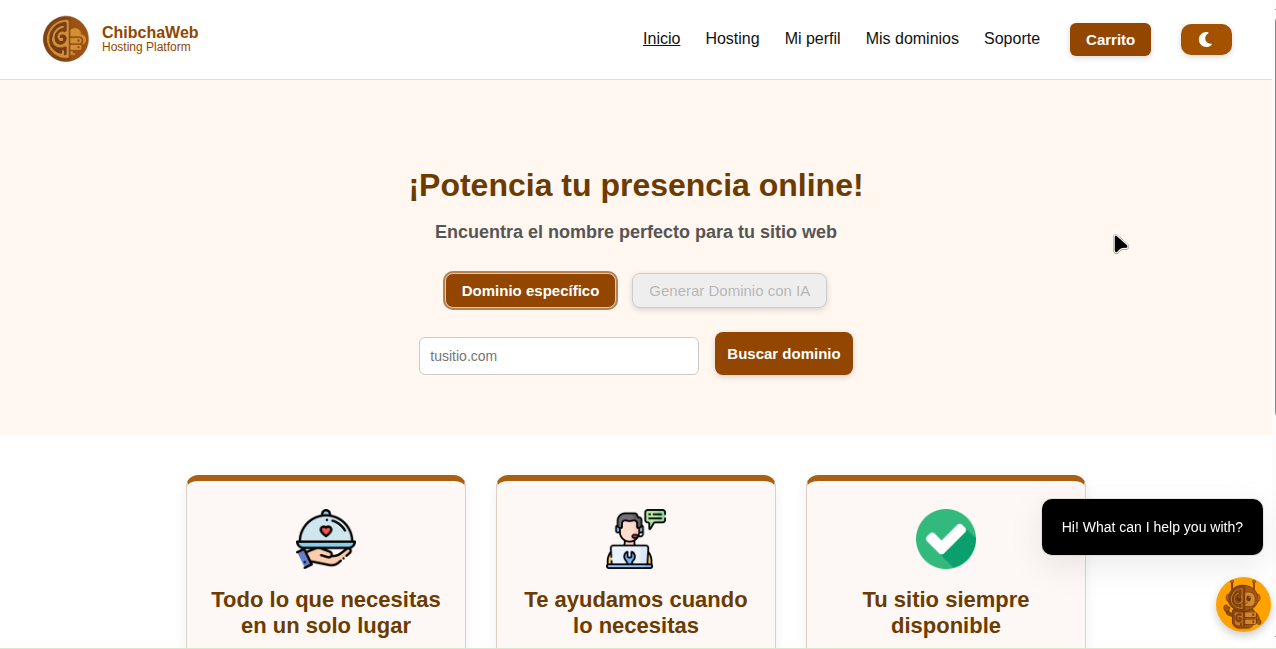
\includegraphics[width=\columnwidth]{acceso/inicio.png}
	\caption{Página principal.}
	\label{fig:inicio}
\end{figure}

\subsection{Registro de usuario }
Sin embargo, para comprar un dominio, será necesario registrarse de la siguiente manera:

\begin{enumerate}
	\item Dar Click en el botón de “Mi perfil”
	\begin{figure}[H]
		
\includegraphics[width=\columnwidth]{acceso/navbar-perfil.png}
		\caption{Barra de navegación.}
		\label{fig:navbar-perfil}
	\end{figure}
	\item Decidir qué tipo de registro se desea (Cliente o distribuidor)
   	\begin{figure}[H]
        \centering
  		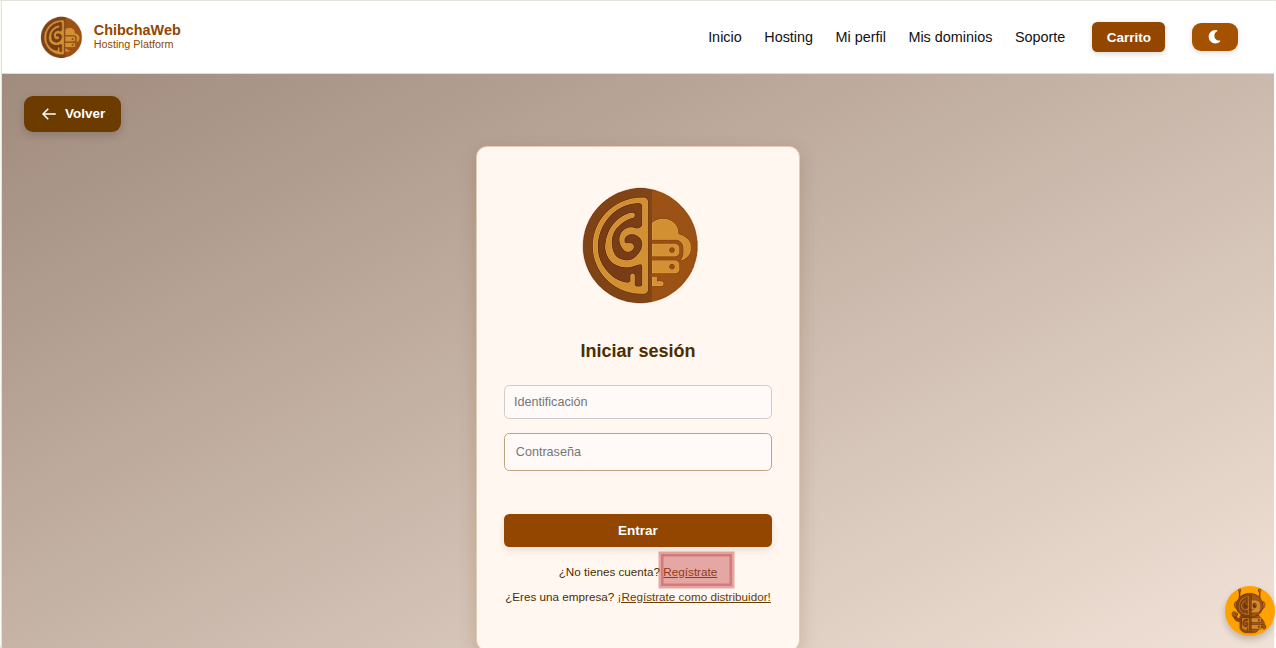
\includegraphics[width=\columnwidth]{acceso/login-registro.png}
  		\caption{Login.}
  		\label{fig:login-registrol}
   	\end{figure}
    \begin{enumerate}
        \item Si su registro es cómo cliente, llene el formulario siguiente:
        \begin{figure}[H]
            \centering
      		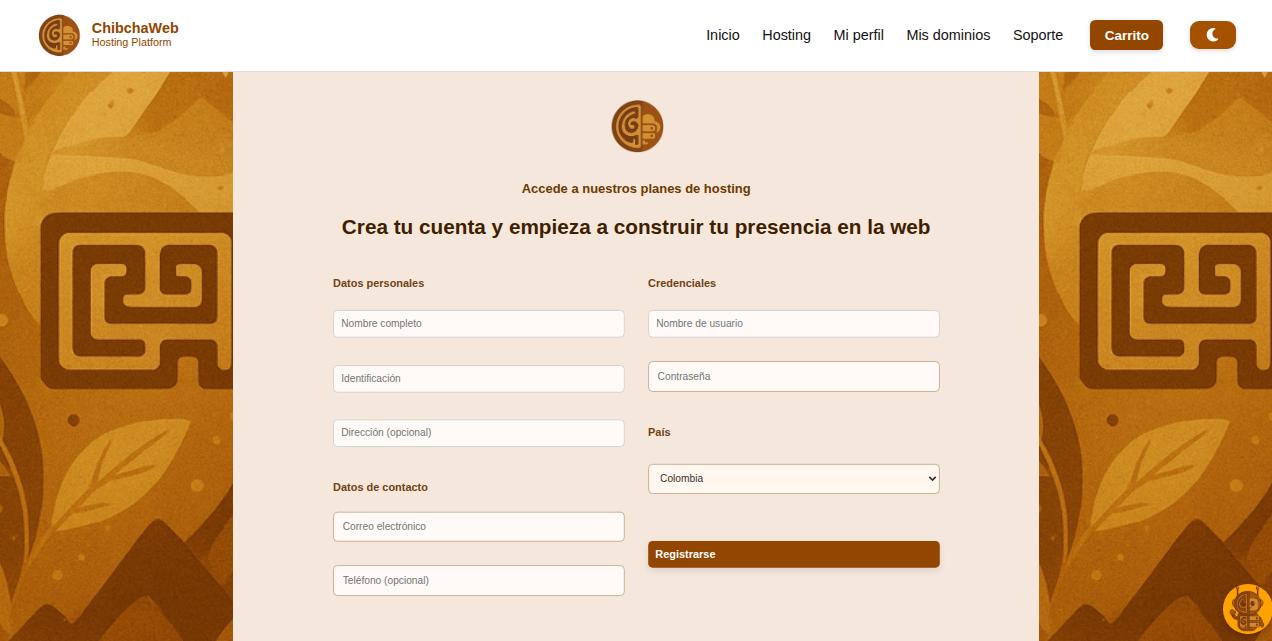
\includegraphics[width=\columnwidth]{acceso/registro-cliente.png}
      		\caption{Registro cliente.}
      		\label{fig:registro-cliente}
       	\end{figure}
        \item Si su registro es cómo distribuidor, llene el formulario siguiente:
        \begin{figure}[H]
            \centering
      		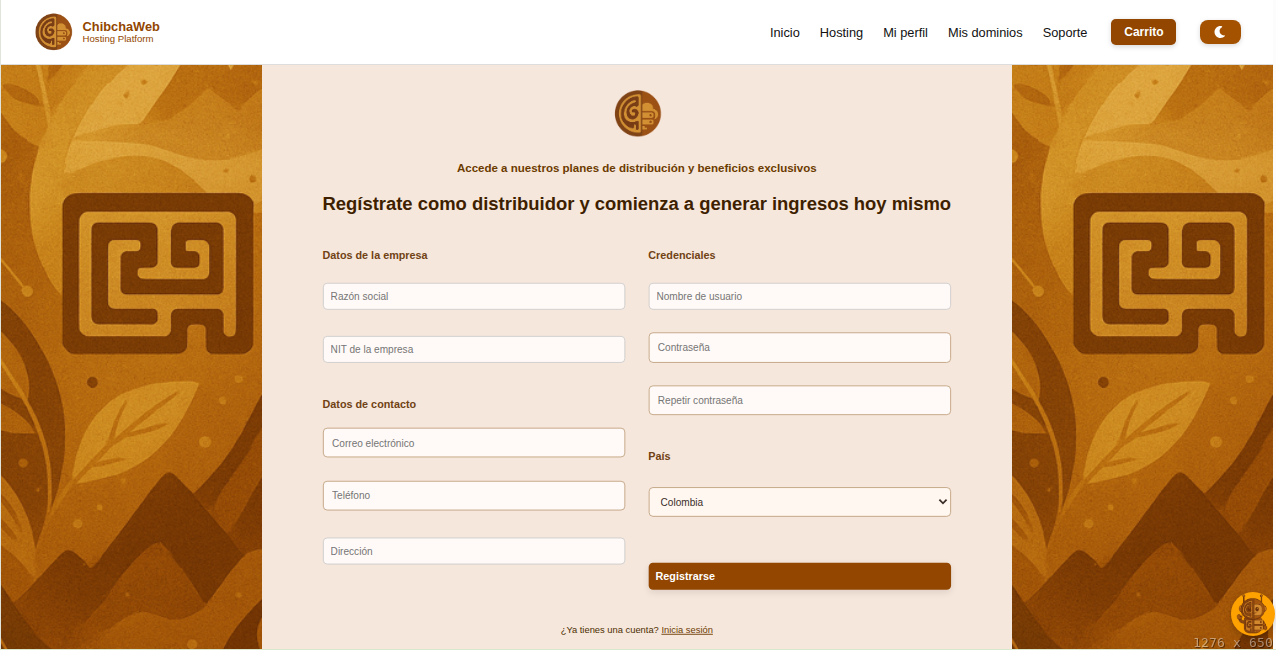
\includegraphics[width=\columnwidth]{acceso/registro-distribuidor.png}
      		\caption{Registro distribuidor.}
      		\label{fig:registro-distribuidor}
       	\end{figure}
    \end{enumerate}
    \item En ambos casos de click en el botón “Registrarse”
    \item Se enviará un código de verificación a su correo electrónico.
    \begin{figure}[H]
        \centering
  		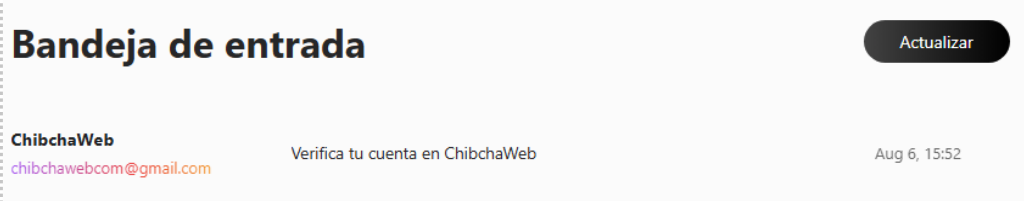
\includegraphics[width=\columnwidth]{acceso/email-verificacion.png}
  		\caption{Email de verificación.}
  		\label{fig:email-verificacion}
   	\end{figure}
    \item Deberá ingresar el código de verificación al siguiente espacio, y dar click en “confirmar”.
    \begin{figure}[H]
        \centering
  		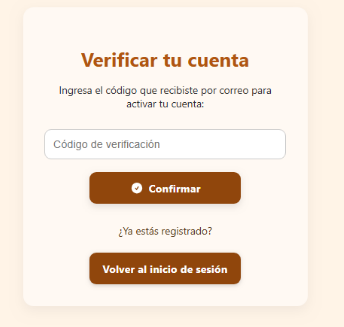
\includegraphics[width=10cm]{acceso/confirmar.png}
  		\caption{Confirmación email.}
  		\label{fig:confirmar}
   	\end{figure}
\end{enumerate}

Luego de esto será redirigido al inicio de sesión.

\subsection{Inicio de sesión}
Para el inicio de sesión, deberá ingresar su identificador de usuario, y su contraseña en los espacios que se ven en la Figura \ref{fig:login-registrol} En caso de no contar con una cuenta, revise el punto anterior.

Luego de clic en entrar, donde deberá ver una interfaz similar a la siguiente
